%%%%%%%%%%%%%%%%%%%%%%%%%%%%%%%%%%%%%%%%%%%%%%%%%%%%%%%%%%%%%%%%%%%%%%%%%
\section{Theoretical Results}  %%%%%%%%%%%%%%%%%%%%%%%%%%%%%%%%%%%%%%%%%%
\label{rs:sec:theory}

In this section, we begin by studying the behavior and output of Quicksort under inconsistent comparison outcomes, without any assumptions on the noise generating process.
Then, starting in Section~\ref{rs:sec:poisson}, we focus on comparison outcomes generated by the BT model.
For clarity, longer proofs are deferred to Section~\ref{rs:sec:proofs}.

\begin{algorithm}[t]
   \caption{Quicksort.}
   \label{rs:alg:quicksort}
\begin{algorithmic}[1]
   \Require set of items $\mathcal{V} \subseteq [N]$
   \OneLineIf{$\Abs{\mathcal{V}} < 2$} \Return list($\mathcal{V}$)
   \Comment{Terminating case.}
   \State $\mathcal{L} \gets \varnothing, \mathcal{R} \gets \varnothing$
   \State $p \gets $ element of $\mathcal{V}$ selected uniformly at random \label{rs:line:pivot}
   \For{$i \in \mathcal{V} \setminus \{ p \}$} \label{rs:line:startpart}
     \If{$i \prec p$} \label{rs:line:comp}
     \Comment{Pairwise comparison.}
       \State $\mathcal{L} \gets \mathcal{L} \cup \{i\}$
     \Else
       \State $\mathcal{R} \gets \mathcal{R} \cup \{i\}$
     \EndIf
   \EndFor  \label{rs:line:stoppart}
   \State \Return $\text{Quicksort}(\mathcal{L}) \cdot p \cdot \text{Quicksort}(\mathcal{R})$ \label{rs:line:return}
\end{algorithmic}
\end{algorithm}

Quicksort (Algorithm~\ref{rs:alg:quicksort}) is best described as a recursive procedure.
At each step of the recursion, a \emph{pivot} item $p$ is chosen uniformly at random (line \ref{rs:line:pivot}).
Then, during the \emph{partition} operation (lines \ref{rs:line:startpart}--\ref{rs:line:stoppart}), every other item is compared to $p$ and added to the set $\mathcal{L}$ or $\mathcal{R}$, depending on the outcome of the comparison with the pivot.
If all comparison outcomes are consistent, it is well-known that Quicksort terminates after sampling \BigO{N \log N} comparisons with high probability.
What happens if we drop the consistency assumption?
The following two lemmas state that these key properties remain valid, no matter which (and how many) comparison outcomes are inconsistent.

\begin{lemma}
\label{rs:lem:termination}
Quicksort always terminates and samples each of the $N(N\!-\!1) / 2$ possible comparisons at most once.
\end{lemma}

\begin{proof}
The proof is identical to the consistent setting.
Consider the state of $\mathcal{L}$ and $\mathcal{R}$ at the end of a partition operation.
Because $\Abs{\mathcal{L}} + \Abs{\mathcal{R}} = \Abs{\mathcal{V}} - 1$, the recursive calls are made on sets of items of strictly decreasing cardinality, and the algorithm terminates after a finite number of steps.
Furthermore, suppose that Quicksort samples an outcome for the pair $(i, j)$.
Then either $i$ or $j$ is the pivot in a partition operation.
In either case, the pivot is not included in the recursive calls, which ensures that $(i, j)$ cannot be compared again.
\end{proof}

\begin{lemma}
\label{rs:lem:samplecomp}
%If the comparison outcomes are independent of the query order,
Quicksort samples \BigO{N \log N} comparisons with high probability.
\end{lemma}

\begin{proof}[Proof (sketch).]
We follow a standard analysis of Quicksort \citep[see, e.g.,][Section 3.3.3]{dubhashi2009concentration}.
With high probability, we choose a ``good'' pivot (i.e., one that results in a balanced partition) a constant fraction of the time.
In this case, the depth of the call tree is \BigO{\log N}.
As there are at most $N$ comparisons at each level of the call tree, we conclude that Quicksort uses \BigO{N \log N} comparisons in total.
With respect to the standard proof, ours requires additional work in order to formalize the notion of ``good'' pivot to the setting where comparison outcomes are not consistent with a linear order.
\end{proof}

Lemma~\ref{rs:lem:samplecomp} complements Theorem~$3$ in \citet{ailon2010preference}, which states that Quicksort samples \BigO{N \log N} in expectation.
These results might suggest that \emph{all} properties of Quicksort carry over to the noisy setting.
This is not the case.
For example, although Quicksort uses approximately $2N \ln N$ comparisons on average in the noiseless setting \citep{sedgewick2011algorithms}, this number can be distinctly different with inconsistent comparison outcomes\footnote{%
E.g., if comparison outcomes are uniformly random, all items are ``good'' pivots with high probability, and the average number of comparisons will be closer to $N \log_2 N$ on average, for large $N$.}.

Quicksort (and efficient sorting algorithms in general) infer most pairs of items' relative position by transitivity and rely heavily on the consistency of comparison outcomes.
In the noisy case, it is therefore important to precisely understand the effect of an inconsistent outcome on the output of the algorithm; this effect extends beyond the pair of items whose comparison outcome was inconsistent.
For this purpose, the next Lemma bounds the displacement of Quicksort's output as a function of the inconsistent outcomes.

\begin{lemma}
\label{rs:lem:dispbound}
Let $\mathcal{E}$ be the set of pairs sampled by Quicksort whose outcome is inconsistent with \Id.
Let $\sigma$ be the output of Quicksort.
Then,
\begin{align*}
\Disp{\sigma} \le 2 \sum_{\mathclap{(i, j) \in \mathcal{E}}}\; \Abs{i - j}
\end{align*}
\end{lemma}

\begin{proof}[Proof (sketch).]
Consider the first partition operation, with pivot $p$, resulting in partitions $\mathcal{L}$ and $\mathcal{R}$.
Denote the set of pairs of items involved in errors made during this partition operation by $\mathcal{E}_1$.
We can show that the displacement is bounded by
\begin{align*}
\Disp{\sigma} \le \Disp[\mathcal{L}]{\sigma} + \Disp[\mathcal{R}]{\sigma} + 2 \;\sum_{\mathclap{(i, j) \in \mathcal{E}_1}} \Abs{i - j},
\end{align*}
where \Disp[\mathcal{L}]{\sigma} and \Disp[\mathcal{R}]{\sigma} represent the displacement of the ordering induced by $\sigma$ on $\mathcal{L}$ and $\mathcal{R}$, respectively.
In other words, the total displacement can be decomposed into a term that represents the ``local'' displacement due to the partition operation and into two terms that account for errors in the recursive calls.
We obtain the desired result by recursively bounding \Disp[\mathcal{L}]{\sigma} and \Disp[\mathcal{R}]{\sigma}.
\end{proof}

Informally, Lemma~\ref{rs:lem:dispbound} states that the displacement can be bounded by a sum of ``local shifts'' due to the inconsistent outcomes and that the price to pay for any information inferred by transitivity is bounded by a factor two.
Lemma~\ref{rs:lem:dispbound} is a crucial component of our subsequent analysis of BT noise, and we believe that it can be useful in order to investigate Quicksort under a wide variety of other noise generating processes.


%%%%%%%%%%%%%%%%%%%%%%%%%%%%%%%%%%%%%%%%%%%%%%%%%%%%%%%%%%%%%%%%%%%%%%%%%
\subsection{Poisson-Distributed Parameters}
\label{rs:sec:poisson}

From here on, we assume that comparison outcomes are generated from $\BT(\bm{\theta})$.
Clearly, any results on the displacement of a ranking estimated from samples of a BT model will depend on $\bm{\theta}$; it is easy to construct a model instance for which it is arbitrarily hard to recover the ranking, by choosing parameters sufficiently close to each other.
Our approach is as follows.
We postulate a family of distributions over $\bm{\theta}$, and we give bounds on the displacement that hold with high probability.

We suppose that comparison outcomes are (in expectation) \emph{uniformly noisy across the ranking}: i.e., comparing two elements at the bottom is (a priori) as difficult as comparing two elements at the top or in the middle.
This means that the probability distribution over parameters $\theta_1, \ldots, \theta_N$ results in (random) distances $\Abs{\theta_{i+k} - \theta_i}$ that depend only on $k$.
One such distribution arises if the parameters are drawn from a Poisson point process of rate $\lambda$.
That is,
\begin{align}
\label{rs:eq:poisson}
\text{i.i.d.}\; x_1, \ldots, x_{N-1} \sim \DExp{\lambda}, \qquad
\theta_i = \sum_{n=1}^{i-1} x_n.
\end{align}
The average distance between two items separated by $k$ positions in the ordering is $\Exp{\theta_{i+k} - \theta_i} = k / \lambda$.
%More generally, the distance \Abs{\theta_{k+i} - \theta_i} has distribution $\DGamma{k, \lambda}$.
Although the distance between adjacent items is constant in expectation, we let some parameters be arbitrarily close\footnote{%
In particular, the expected minimum distance between two items (i.e., the $\min$ of $N$ exponential r.v.s) decreases as $(N\lambda)^{-1}$ as $N$ increases.}.
The parameter $\lambda$ indirectly controls the expected level of noise; a large $\lambda$ is likely to result in a larger number of inconsistent outcomes.
Although the precise choice of this Poisson model is driven by tractability concerns, in Section~\ref{rs:sec:iidunif} we argue that it is essentially equivalent to choosing the parameters independently and uniformly at random in the interval $[0, (N+1) / \lambda]$, when $\lambda$ is fixed and $N$ is large.
We are now ready to state our main result.

\begin{theorem}
\label{rs:thm:quickdisp}
Let $\bm{\theta}$ be sampled from a Poisson point process of rate $\lambda$.
Let $\sigma$ be the output of Quicksort using comparison outcomes sampled from $\BT(\bm{\theta})$.
Then,
\begin{align}
\Disp{\sigma}
    &= \BigO{ \lambda^2 N }, \label{rs:eq:qdtot} \\
\max_{i} \; \Abs{\sigma(i) - i}
    &= \BigO{ \lambda \log N }, \label{rs:eq:qdmax}
\end{align}
with high probability.
\end{theorem}

\begin{proof}[Proof (sketch)]
Let $z_{ij}$ be the indicator random variable of the event ``the comparison between $i$ and $j$ results in an error'', and let $d_{ij} = \Abs{\theta_i - \theta_j}$.
The distance $d_{ij}$ is a sum of $\Abs{i - j}$ i.i.d. exponential random variables, i.e., $d_{ij} \sim \DGamma{\Abs{i - j}, \lambda}$, and we can show that
\begin{align*}
\Exp{z_{ij}} &= \Exp{\frac{1}{1 + \exp(d_{ij})}}
    \le \Exp{\exp(-d_{ij})} = (1 + 1/\lambda)^{-\Abs{i - j}}.
\end{align*}
Using Lemma~\ref{rs:lem:dispbound} and the fact that every pair of items is compared at most once, we find
\begin{align*}
\Exp{\Delta}
    \le 2 \sum_{i < j}\; \Abs{i - j} \Exp{z_{ij}}
    \le 2N \sum_{k = 0}^{\infty} k (1 + 1/\lambda)^{-k} = 2N \lambda (\lambda + 1).
\end{align*}
The random variables $\{ z_{ij} \}$ are not independent (they are independent when conditioned on $\bm{\theta}$) but, with some more work, we can show that $\Var{\Delta} = \BigO{N}$.
By using a Chebyshev bound, \eqref{rs:eq:qdtot} follows.

In order to prove \eqref{rs:eq:qdmax}, we take advantage of a theorem due to \citet{ailon2008reconciling} which states that
\begin{align*}
\Prob{ \sigma(i) < \sigma(j) \mid \bm{\theta} } = \Prob{i \prec j \mid \bm{\theta}},
\end{align*}
even if $i$ and $j$ were not directly compared with each other.
We use a Chernoff bound on $d_{ij}$ to show that the relative order between any two items separated by at least $\BigO{\lambda \log N}$ positions is correct with high probability.
The second part of the claim follows easily.
\end{proof}

Note that any method that compares each pair of items at most once results in a ranking estimate $\tau$ with displacement $\Disp{\tau} = \BigOmega{N}$ with high probability: As there is only a single (possibly inconsistent) comparison outcome between each pair of adjacent items, it is likely that a constant fraction of the items will be ranked incorrectly, resulting in a displacement that grows linearly in $N$.
Hence, our bound on \Disp{\sigma} shows that Quicksort is order-optimal (in $N$).

In light of Theorem~\ref{rs:thm:quickdisp}, a natural question to ask is as follows.
How many comparisons are needed in order to find the correct ranking?
Finding the exact ranking is difficult: in fact, \BigOmega{N} comparison outcomes are necessary in order to discriminate the closest pair of items reliably, as we show next.
Suppose that we are given $K$ comparisons to find the relative order between $i$ and $j$, and define $e_{ij}$ as the event ``more than half of the $K$ comparison outcomes between $i$ and $j$ are inconsistent''.

\begin{proposition}
Let $\bm{\theta}$ be sampled from a Poisson point process of rate $\lambda$.
Then, there is a pair $i, j \in [N]$ and a constant $c > 0$ independent of $N$ such that if $K = \LittleO{\lambda N}$,
\begin{align*}
\Prob{e_{ij}} \ge c
\end{align*}
with high probability.
\end{proposition}

\begin{proof}
The distance between the two closest items is $d_{\min} = \min_i \Abs{\theta_{i+1} - \theta_{i}} = \min_n x_n$, i.e., the minimum of $N-1$ independent exponential random variables of rate $\lambda$.
Therefore, $d_{\min} \sim \DExp{(N-1)\lambda}$, and for $N \ge 2$ with probability at least $1 - e^{-1/2} \approx 0.39$ we have $d_{\min} \le (\lambda N)^{-1}$.
Let $z_k$ be the indicator random variable for the event ``the outcome of the $k$-th comparison is incorrect''.
Assuming that $d_{\min} \le (\lambda N)^{-1}$ and that $\lambda N \ge 1/2$,
\begin{align*}
\Prob{z_k = 0}
    &\le \frac{1}{1 + \exp[-1 / (\lambda N)]} \le \frac{1}{2 - 1/(\lambda N)}
     = \frac{1}{2} \cdot \left( 1 + \frac{1}{2\lambda N - 1} \right) \\
    &\le \frac{1}{2} \exp \left[ \frac{1}{2\lambda N - 1} \right],
\end{align*}
where we used the inequality $e^{x} \ge 1 + x$ twice.
The probability of \emph{correctly} identifying the relative order between the two closest items based on $K$ comparisons is
\begin{align*}
\Prob{\sum_{k = 1}^K z_k \le K/2}
    &\le \sum_{\ell = 1}^{K/2} \binom{K}{\ell} \Prob{z_k = 0}^K
     \le \exp \left[ \frac{K}{2\lambda N - 1} \right] \cdot 2^{-K} \sum_{\ell = 1}^{K/2} \binom{K}{\ell} \\
    &= \frac{1}{2} \exp \left[ \frac{K}{2\lambda N - 1} \right].
\end{align*}
As $\Prob{e_{ij}} = 1 - \Prob{\sum_{k = 1}^K z_k \le K/2}$, it follows that, if $K = \LittleO{\lambda N}$, the probability of \emph{incorrectly} identifying the relative order between the two closest items is bounded from below by a positive constant.
\end{proof}

As finding the \emph{exact} ranking appears to be difficult, we instead focus on finding a ranking that matches the ground truth everywhere, except at a vanishing fraction of the items.

\begin{algorithm}[t]
   \caption{Multisort.}
   \label{rs:alg:multisort}
\begin{algorithmic}[1]
   \Require set of items $\mathcal{V} \subseteq [N]$, number of iterations $K$
   \State $\mathcal{S} \gets \varnothing$
   \For{$k = 1, \ldots, K$}
     \State $\sigma \gets \text{Quicksort}(\mathcal{V})$
     \State $\mathcal{S} \gets \mathcal{S} \cup \{ \sigma \}$
   \EndFor
   \State \Return Copeland aggregation of $\mathcal{S}$
\end{algorithmic}
\end{algorithm}

Multiple runs of Quicksort likely produce different outputs, because of the noisy comparison outcomes and because the algorithm itself is randomized (the pivot selection is random).
By aggregating $K$ independent outputs of Quicksort, is it possible to produce a better ranking estimate?
Similarly to \citet{szorenyi2015online}, we combine the $K$ outputs  $\sigma_1, \ldots, \sigma_K$ into an aggregate ranking $\hat{\sigma}$ using Copeland's method.
The method assigns, to each item, a score that corresponds to the number of items that it beats in a majority of the rankings, and it then ranks the items by increasing score \citep{copeland1951reasonable}.
We call the procedure Multisort and describe it in Algorithm~\ref{rs:alg:multisort}.

\begin{theorem}
\label{rs:thm:multidisp}
Let $\bm{\theta}$ be sampled from a Poisson point process of rate $\lambda$.
Let $\hat{\sigma}$ be the output of Multisort using $K = \BigO{\lambda^2 \log^5 N}$ and comparison outcomes sampled from $\BT(\bm{\theta})$.
Then,
\begin{align*}
\Disp{\hat{\sigma}} = \LittleO{\lambda N}
\end{align*}
with high probability.
\end{theorem}

\begin{proof}[Proof (sketch)]
We use results on the order statistics of the distances $x_1, \ldots, x_{N-1}$ between successive items, as defined in \eqref{rs:eq:poisson}, to partition the items into two disjoint subsets $\mathcal{B}$ and $\mathcal{G}$.
The set $\mathcal{B}$ contains a vanishing $(1/\log^2 N)$-fraction of ``bad'' items that are difficult to order.
The set $\mathcal{G}$ is such that the smallest distance $d_{ij}$ from any item $i \in \mathcal{G}$ to any other item $j \in [N]$ is bounded from below by $c / (\lambda \log^2 N)$.
We can show that with $K = \BigO{\lambda^2 \log^5 N}$, for any $i \in \mathcal{G}$ and $j \in [N]$ we have $i < j \iff \sigma(i) < \sigma(j)$ in a majority of the Quicksort outputs (with high probability).
This implies that $\hat{\sigma}(i) = i$ for all $i \in \mathcal{G}$ with high probability.
Using \eqref{rs:eq:qdmax} for items in $\mathcal{B}$, we have
\begin{align*}
\Disp{\hat{\sigma}} = \Abs{\mathcal{B}} \cdot \BigO{\lambda \log N} = \BigO{\lambda N / \log N}
\end{align*}
with high probability.
\end{proof}

Theorem~\ref{rs:thm:multidisp} states that all but a vanishing fraction of items are correctly ranked using \BigO{\lambda^2 N \log^6 N} comparisons.
This result should be compared to that of \citet{rajkumar2014statistical} obtained in the passive setting, which suggests that \BigOmega{N^2} comparisons are needed if samples are selected uniformly at random.

\paragraph{Empirical Validation}

In Figure~\ref{rs:fig:bounds}, we illustrate Theorems~\ref{rs:thm:quickdisp} and~\ref{rs:thm:multidisp} by running simulations for increasing $N$ and different values of $\lambda$.
The bound on \Disp{\sigma} is tight in $N$, but the dependence on $\lambda$ appears to be linear rather than quadratic.
The bound on $\max_i \Abs{\sigma(i) - i}$ appears to be tight in $N$ and $\lambda$.
Finally, we compare the Copeland aggregation of $K$ outputs of Quicksort with the ranking induced by the maximum-likelihood estimate (MLE), inferred from the outcomes of all the pairwise comparisons sampled by the $K$ runs.
Although the ranking induced by the MLE does not benefit from the guarantees of Theorem~\ref{rs:thm:multidisp}, it performs better in practice.
We will make use of this observation in Section~\ref{rs:sec:experiments}.

\begin{figure}[p]
\centering
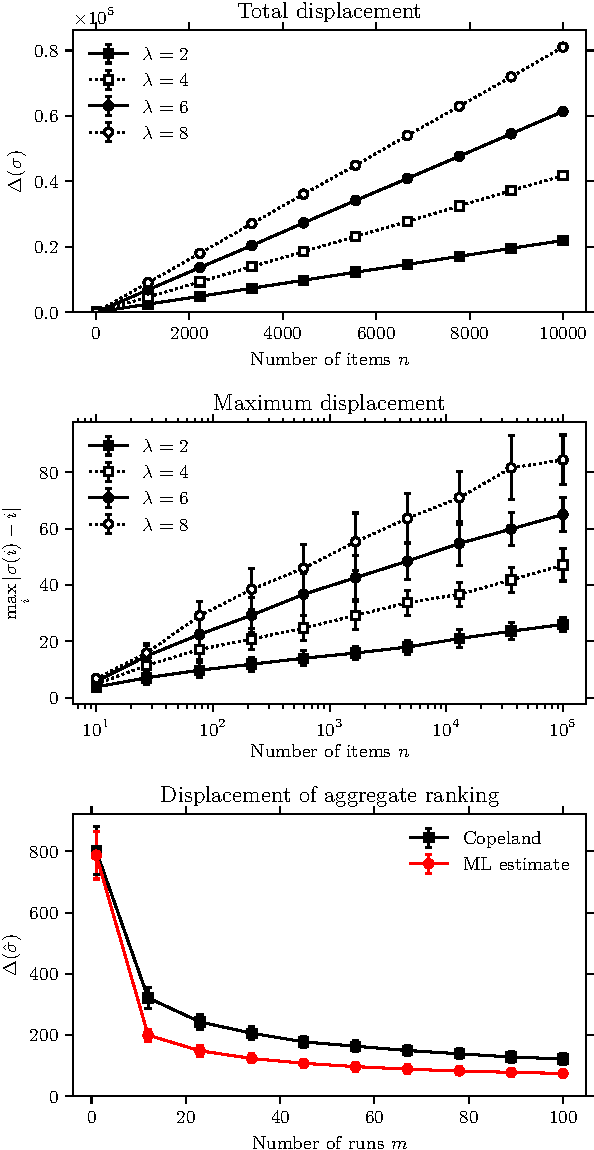
\includegraphics{rs-bounds}
\caption{
Empirical validation of Theorem~\ref{rs:thm:quickdisp} and illustration of Theorem~\ref{rs:thm:multidisp}.
Every simulation is repeated $50$ times, and we report the mean and the standard deviation.
Top and middle: total and maximum displacement (respectively) for increasing $N$ and different values of $\lambda$.
Bottom: displacement of the aggregate ranking $\hat{\sigma}$ for increasing $K$, fixing $N = \num{200}$ and $\lambda = \num{4}$ and using two different aggregation rules.
}
\label{rs:fig:bounds}
\end{figure}


%%%%%%%%%%%%%%%%%%%%%%%%%%%%%%%%%%%%%%%%%%%%%%%%%%%%%%%%%%%%%%%%%%%%%%%%%
\subsection{Independent Uniformly Distributed Parameters}
\label{rs:sec:iidunif}

A different (perhaps more natural) assumption about the parameters $\bm{\theta}$ is to consider that they are drawn independently and uniformly at random over some interval.
That is,
\begin{align*}
\text{i.i.d.}\; \bar{\theta}_1, \ldots, \bar{\theta}_N \sim \DUnif{0, (N+1) / \lambda},
\end{align*}
with $\theta_1, \ldots, \theta_N$ the order statistics of $\bar{\bm{\theta}}$, i.e., the random variables arranged in increasing order.
From some elementary results on the joint distribution of order statistics \citep[see, e.g.,][]{arnold2008first}, we have that
\begin{align*}
\Abs{\theta_{i+k} - \theta_{i}} \sim (N+1) / \lambda \cdot \DBeta{k, N - k + 1},
\end{align*}
i.e., $\Abs{\theta_{i+k} - \theta_{i}}$ is distributed as a Beta random variable rescaled between $0$ and $(N+1) / \lambda$.
Letting $f_{k,N}(x)$ be the probability density of $\Abs{\theta_{i+k} - \theta_{i}}$, we have, for any fixed $k$ and $\lambda$,
\begin{align*}
f_{k,N}(x) \propto x^{k-1} \left[ 1 - \frac{\lambda x}{N + 1} \right]^{N - k} \xrightarrow{N \to \infty} x^{k-1} e^{-\lambda x}.
\end{align*}
We recognize the functional form of the density of a \DGamma{k, \lambda} distribution.
Hence, the Poisson model and the i.i.d. uniform model are essentially equivalent for fixed $\lambda$ and large $N$, and we can expect the results developed in Section~\ref{rs:sec:poisson} to hold in the i.i.d. uniform case as well.
